\section{Pruebas de Casos de Uso principales}
La aplicación móvil se compone de nueve vistas principales:
\begin{itemize}
 \item Configuración Personal
 \item Hoteles
 \item Vuelos
 \item Info AICM
 \item Lista de Equipaje
 \item Itinerario de viaje
 \item Ruta al AICM
 \item Ubícate
 \item Info Vuelo
\end{itemize}

A su vez cada módulo puede desplegar información diversa en otras vistas o en su caso a partir opciones adicionales sobre un menú 
secundario.
\subsection{Configuración Personal}

\definecolor{blanco}{RGB}{255,255,255}

\begin{table}[h]
	\begin{center}
		\begin{tabular}{|>{\color{blanco}}c|>{\color{blanco}}c|>{\color{blanco}}c|>{\color{blanco}}c|}
			\hline \rowcolor[RGB]{51,153,255} 
				{\bf CU} & 
				{\bf Acción o evento} &
				{\bf Resultados y/u observaciones} &
				{\bf } \\
			\hline 
				\multicolumn{1}{|m{1.8cm}|}{\centering CU-U-01} &
				\multicolumn{1}{m{4.5cm}|}{\centering Clic normal en crear configuración} &
				\multicolumn{1}{m{5.5cm}|}{\centering Se ingresan datos como email, clase de
				viaje y categoría de hotel por número de estrellas.El registro en el web service es exitoso.} &
				\multicolumn{1}{m{1.5cm}|}{\centering 
\includegraphics[width=8mm, height=8mm]{Figuras/palomita.png}} \\
      		\hline \rowcolor[RGB]{240,248,255} 
				\multicolumn{1}{|m{1.8cm}|}{\centering CU-U-01} &
				\multicolumn{1}{m{4.5cm}|}{\centering Clic normal en evitar configuración} &
				\multicolumn{1}{m{5.5cm}|}{\centering Se muestra el menú principal de TASMC y la opción de configurar sobre un 
				menú secundario.} &
				\multicolumn{1}{m{1.5cm}|}{\centering 
\includegraphics[width=8mm, height=8mm]{Figuras/palomita.png}} \\
		\hline 
				\multicolumn{1}{|m{1.8cm}|}{\centering CU-U-01} &
				\multicolumn{1}{m{4.4cm}|}{\centering Clic normal en opción de reconfiguración} &
				\multicolumn{1}{m{5.5cm}|}{\centering Se ingresan los datos de email, clase de viaje y categoría de 
				hotel. La fecha de configuración del usuario es modificada dentro del web service de administración.} &
				\multicolumn{1}{m{1.5cm}|}{\centering 
\includegraphics[width=8mm, height=8mm]{Figuras/palomita.png}} \\
      		\hline 
		\end{tabular}
	\end{center}
	\caption[Pruebas del módulo de Configuración Personal} 
	\label{tab:pruebasConfiguracion}
\end{table}
\clearpage

\subsection{Hoteles}

\definecolor{blanco}{RGB}{255,255,255}

\begin{table}[h]
	\begin{center}
		\begin{tabular}{|>{\color{blanco}}c|>{\color{blanco}}c|>{\color{blanco}}c|>{\color{blanco}}c|}
			\hline \rowcolor[RGB]{51,153,255} 
				{\bf CU} & 
				{\bf Acción o evento} &
				{\bf Resultados y/u observaciones} &
				{\bf } \\
			\hline 
				\multicolumn{1}{|m{1.8cm}|}{\centering CU-U-02} &
				\multicolumn{1}{m{4.5cm}|}{\centering Clic normal en búsqueda de hoteles} &
				\multicolumn{1}{m{5.5cm}|}{\centering Despliega la información de hoteles correspondiente a las parámetros ingresados 
				en el formulario.} &
				\multicolumn{1}{m{1.5cm}|}{\centering 
\includegraphics[width=8mm, height=8mm]{Figuras/palomita.png}} \\
      		\hline \rowcolor[RGB]{240,248,255} 
				\multicolumn{1}{|m{1.8cm}|}{\centering CU-U-02} &
				\multicolumn{1}{m{4.5cm}|}{\centering Clic normal en filtrado por precio} &
				\multicolumn{1}{m{5.5cm}|}{\centering Se organiza la información de hoteles de menor a mayor precio.} &
				\multicolumn{1}{m{1.5cm}|}{\centering 
\includegraphics[width=8mm, height=8mm]{Figuras/palomita.png}} \\
		\hline 
				\multicolumn{1}{|m{1.8cm}|}{\centering CU-U-02} &
				\multicolumn{1}{m{4.5cm}|}{\centering Clic normal en filtrado por número de estrellas} &
				\multicolumn{1}{m{5.5cm}|}{\centering Se organiza la información de hoteles de menor a mayor número de estrellas.} &
				\multicolumn{1}{m{1.5cm}|}{\centering 
\includegraphics[width=8mm, height=8mm]{Figuras/palomita.png}} \\
      		\hline \rowcolor[RGB]{240,248,255} 
				\multicolumn{1}{|m{1.8cm}|}{\centering CU-U-02} &
				\multicolumn{1}{m{4.5cm}|}{\centering Arrastrar lista de hoteles para actualización} &
				\multicolumn{1}{m{5.5cm}|}{\centering Se deja presionada la lista de hoteles y se arrastra hacia abajo 
				para actualizar la información. No se muestran nuevos resultados con dichos paramétros.} &
				\multicolumn{1}{m{1.5cm}|}{\centering 
\includegraphics[width=8mm, height=8mm]{Figuras/palomita.png}} \\
      		        \hline 
      		        
		\end{tabular}
	\end{center}
	\caption[Pruebas del módulo de Hoteles} 
	\label{tab:pruebasHoteles}
\end{table}
\clearpage

\subsection{Vuelos}

\definecolor{blanco}{RGB}{255,255,255}

\begin{table}[h]
	\begin{center}
		\begin{tabular}{|>{\color{blanco}}c|>{\color{blanco}}c|>{\color{blanco}}c|>{\color{blanco}}c|}
			\hline \rowcolor[RGB]{51,153,255} 
				{\bf CU} & 
				{\bf Acción o evento} &
				{\bf Resultados y/u observaciones} &
				{\bf } \\
			\hline 
				\multicolumn{1}{|m{1.8cm}|}{\centering CU-U-03} &
				\multicolumn{1}{m{4.5cm}|}{\centering Clic normal en búsqueda de vuelos de ida} &
				\multicolumn{1}{m{5.5cm}|}{\centering Despliega la información correspondiente de vuelos de ida según los parámetros ingresados 
				en el formulario de ida.} &
				\multicolumn{1}{m{1.5cm}|}{\centering 
\includegraphics[width=8mm, height=8mm]{Figuras/palomita.png}} \\
      		\hline \rowcolor[RGB]{240,248,255} 
      				\multicolumn{1}{|m{1.8cm}|}{\centering CU-U-03} &
				\multicolumn{1}{m{4.5cm}|}{\centering Clic normal en búsqueda de vuelos redondos} &
				\multicolumn{1}{m{5.5cm}|}{\centering Despliega la información correspondiente de vuelos de ida y vuelta según los parámetros ingresados 
				en el formulario de ida/vuelta.} &
				\multicolumn{1}{m{1.5cm}|}{\centering 
\includegraphics[width=8mm, height=8mm]{Figuras/palomita.png}} \\
      		\hline 
				\multicolumn{1}{|m{1.8cm}|}{\centering CU-U-03} &
				\multicolumn{1}{m{4.5cm}|}{\centering Clic normal en filtrado por precio} &
				\multicolumn{1}{m{5.5cm}|}{\centering Se organiza la información de vuelos de menor a mayor precio.} &
				\multicolumn{1}{m{1.5cm}|}{\centering 
\includegraphics[width=8mm, height=8mm]{Figuras/palomita.png}} \\
		\hline \rowcolor[RGB]{240,248,255} 
				\multicolumn{1}{|m{1.8cm}|}{\centering CU-U-03} &
				\multicolumn{1}{m{4.5cm}|}{\centering Clic normal en filtrado por fecha de vuelo} &
				\multicolumn{1}{m{5.5cm}|}{\centering Se organiza la información de vuelos por fecha de ida y vuelta más cercanos.} &
				\multicolumn{1}{m{1.5cm}|}{\centering 
\includegraphics[width=8mm, height=8mm]{Figuras/palomita.png}} \\
      		\hline 
				\multicolumn{1}{|m{1.8cm}|}{\centering CU-U-03} &
				\multicolumn{1}{m{4.5cm}|}{\centering Arrastrar lista de vuelos para actualización} &
				\multicolumn{1}{m{5.5cm}|}{\centering Se deja presionada la lista de vuelos y se arrastra hacia abajo 
				para actualizar la información. No se muestran nuevos resultados con dichos paramétros.} &
				\multicolumn{1}{m{1.5cm}|}{\centering 
\includegraphics[width=8mm, height=8mm]{Figuras/palomita.png}} \\
      		        \hline 
    		\end{tabular}
	\end{center}
	\caption[Pruebas del módulo de Vuelos} 
	\label{tab:pruebasVuelos}
\end{table}

\clearpage

\subsection{Info AICM}

\definecolor{blanco}{RGB}{255,255,255}

\begin{table}[h]
	\begin{center}
		\begin{tabular}{|>{\color{blanco}}c|>{\color{blanco}}c|>{\color{blanco}}c|>{\color{blanco}}c|}
			\hline \rowcolor[RGB]{51,153,255} 
				{\bf CU} & 
				{\bf Acción o evento} &
				{\bf Resultados y/u observaciones} &
				{\bf } \\
			\hline 
				\multicolumn{1}{|m{1.8cm}|}{\centering CU-U-04} &
				\multicolumn{1}{m{4.5cm}|}{\centering Clic normal en Info AICM} &
				\multicolumn{1}{m{5.5cm}|}{\centering Despliega la información del AICM como sitio web, teléfono, ubicación, y dos botones para 
				el mapa y los servicios.} &
				\multicolumn{1}{m{1.5cm}|}{\centering 
\includegraphics[width=8mm, height=8mm]{Figuras/palomita.png}} \\
      		\hline \rowcolor[RGB]{240,248,255} 
      				\multicolumn{1}{|m{1.8cm}|}{\centering CU-U-04} &
				\multicolumn{1}{m{4.5cm}|}{\centering Clic normal en mapa de AICM} &
				\multicolumn{1}{m{5.5cm}|}{\centering Se muestra una vista dividida en planta baja y alta, la cuál 
				puede ser intercambiada mediante un deslizamiento en la pantalla de izquierda a derecha.} &
				\multicolumn{1}{m{1.5cm}|}{\centering 
\includegraphics[width=8mm, height=8mm]{Figuras/palomita.png}} \\
		\hline 
				\multicolumn{1}{|m{1.8cm}|}{\centering CU-U-04} &
				\multicolumn{1}{m{4.5cm}|}{\centering Clic normal en servicios del AICM} &
				\multicolumn{1}{m{5.5cm}|}{\centering Se una lista de los servicios que ofrece el AICM-T1.} &
				\multicolumn{1}{m{1.5cm}|}{\centering 
\includegraphics[width=8mm, height=8mm]{Figuras/palomita.png}} \\
      		        \hline 
    		\end{tabular}
	\end{center}
	\caption[Pruebas del módulo de Info AICM} 
	\label{tab:pruebasInfoAICM}
\end{table}

\clearpage

\subsection{Lista de Equipaje}

\definecolor{blanco}{RGB}{255,255,255}

\begin{table}[h]
	\begin{center}
		\begin{tabular}{|>{\color{blanco}}c|>{\color{blanco}}c|>{\color{blanco}}c|>{\color{blanco}}c|}
			\hline \rowcolor[RGB]{51,153,255} 
				{\bf CU} & 
				{\bf Acción o evento} &
				{\bf Resultados y/u observaciones} &
				{\bf } \\
			\hline 
				\multicolumn{1}{|m{1.8cm}|}{\centering CU-U-05} &
				\multicolumn{1}{m{4.5cm}|}{\centering Clic normal en Lista de Equipaje} &
				\multicolumn{1}{m{5.5cm}|}{\centering Se despliega una lista de equipajes los cuales pueden ser sugerencias 
				cargadas directamente desde el web service o listas creadas por el usuario. Se muestra un mensaje solicitando al usuario 
				conectarse a internet en caso de no tener encendido ese servicio. No carga las sugerencias de equipajes 
				si no se encuentra conectado a internet.} &
				\multicolumn{1}{m{1.5cm}|}{\centering 
\includegraphics[width=8mm, height=8mm]{Figuras/palomita.png}} \\
      		\hline \rowcolor[RGB]{240,248,255} 
      				\multicolumn{1}{|m{1.8cm}|}{\centering CU-U-05} &
				\multicolumn{1}{m{4.5cm}|}{\centering Clic normal en botón de nuevo equipaje} &
				\multicolumn{1}{m{5.5cm}|}{\centering Se muestra un vista donde se debe ingresar un nombre para la lista de 
				equipaje asi como una lista con los objetos que desee llevar en su viaje.} &
				\multicolumn{1}{m{1.5cm}|}{\centering 
\includegraphics[width=8mm, height=8mm]{Figuras/palomita.png}} \\
		\hline 
				\multicolumn{1}{|m{1.8cm}|}{\centering CU-U-05} &
				\multicolumn{1}{m{4.5cm}|}{\centering Clic normal en lista de equipaje} &
				\multicolumn{1}{m{5.5cm}|}{\centering Se muestran una lista con los objetos en el equipaje, mediante 
				la cuál es posible verificar los mismos a la hora de viajar.} &
				\multicolumn{1}{m{1.5cm}|}{\centering 
\includegraphics[width=8mm, height=8mm]{Figuras/palomita.png}} \\
		\hline \rowcolor[RGB]{240,248,255} 
      				\multicolumn{1}{|m{1.8cm}|}{\centering CU-U-05} &
				\multicolumn{1}{m{4.5cm}|}{\centering Clic normal en editar equipaje} &
				\multicolumn{1}{m{5.5cm}|}{\centering Se muestra un vista donde es posible agregar o eliminar objetos del equipaje.} &
				\multicolumn{1}{m{1.5cm}|}{\centering 
\includegraphics[width=8mm, height=8mm]{Figuras/palomita.png}} \\
		\hline 
		      		              		        
    		\end{tabular}
	\end{center}
	\caption[Pruebas del módulo Lista de Equipaje} 
	\label{tab:pruebasEquipaje}
\end{table}

\clearpage

\subsection{Itinerario de viaje}

\definecolor{blanco}{RGB}{255,255,255}

\begin{table}[h]
	\begin{center}
		\begin{tabular}{|>{\color{blanco}}c|>{\color{blanco}}c|>{\color{blanco}}c|>{\color{blanco}}c|}
			\hline \rowcolor[RGB]{51,153,255} 
				{\bf CU} & 
				{\bf Acción o evento} &
				{\bf Resultados y/u observaciones} &
				{\bf } \\
			\hline 
				\multicolumn{1}{|m{1.8cm}|}{\centering CU-U-06} &
				\multicolumn{1}{m{4.5cm}|}{\centering Clic normal en itinerario de Viaje} &
				\multicolumn{1}{m{5.5cm}|}{\centering Se despliega una lista de itinerarios con los itinerarios creados por el usuario, 
				cada uno con información referente al destino y actividades en dicho viaje.} &
				\multicolumn{1}{m{1.5cm}|}{\centering 
\includegraphics[width=8mm, height=8mm]{Figuras/palomita.png}} \\
      		\hline \rowcolor[RGB]{240,248,255} 
      				\multicolumn{1}{|m{1.8cm}|}{\centering CU-U-06} &
				\multicolumn{1}{m{4.5cm}|}{\centering Clic normal sobre un itinerario} &
				\multicolumn{1}{m{5.5cm}|}{\centering Se muestran los detalles del itinerario como es el destino y las actividades a realizar, 
				mismo que puede ser editado.} &
				\multicolumn{1}{m{1.5cm}|}{\centering 
\includegraphics[width=8mm, height=8mm]{Figuras/palomita.png}} \\
		\hline 
				\multicolumn{1}{|m{1.8cm}|}{\centering CU-U-06} &
				\multicolumn{1}{m{4.5cm}|}{\centering Clic normal en nuevo itinerario} &
				\multicolumn{1}{m{5.5cm}|}{\centering Se solicitan los datos del itinerario como es el destino y las 
				actividades a realizar. El itinerario es guardado correctamente en la base de datos.} &
				\multicolumn{1}{m{1.5cm}|}{\centering 
\includegraphics[width=8mm, height=8mm]{Figuras/palomita.png}} \\
		\hline \rowcolor[RGB]{240,248,255} 
      				\multicolumn{1}{|m{1.8cm}|}{\centering CU-U-06} &
				\multicolumn{1}{m{4.5cm}|}{\centering Arrastrar itinerario para eliminación} &
				\multicolumn{1}{m{5.5cm}|}{\centering Se deja presionado el itinerario y se arrastra hacia la derecha para 
				su eliminación. Se elimina correctamente de la base de datos.} &
				\multicolumn{1}{m{1.5cm}|}{\centering 
\includegraphics[width=8mm, height=8mm]{Figuras/palomita.png}} \\
		\hline 
		      		              		        
    		\end{tabular}
    	\end{center}
	\caption[Pruebas del módulo de Itinerario} 
	\label{tab:pruebasItinerario}
\end{table}

\clearpage

\subsection{Ruta al AICM}

\definecolor{blanco}{RGB}{255,255,255}

\begin{table}[h]
	\begin{center}
		\begin{tabular}{|>{\color{blanco}}c|>{\color{blanco}}c|>{\color{blanco}}c|>{\color{blanco}}c|}
			\hline \rowcolor[RGB]{51,153,255} 
				{\bf CU} & 
				{\bf Acción o evento} &
				{\bf Resultados y/u observaciones} &
				{\bf } \\
			\hline 
				\multicolumn{1}{|m{1.8cm}|}{\centering CU-U-07} &
				\multicolumn{1}{m{4.5cm}|}{\centering Clic normal en Ruta AICM} &
				\multicolumn{1}{m{5.5cm}|}{\centering Se despliega un mapa con las distintas localidades de las terminales del AICM. 
				Así como la opción de localización actual.} &
				\multicolumn{1}{m{1.5cm}|}{\centering 
\includegraphics[width=8mm, height=8mm]{Figuras/palomita.png}} \\
      		\hline \rowcolor[RGB]{240,248,255} 
      				\multicolumn{1}{|m{1.8cm}|}{\centering CU-U-07} &
				\multicolumn{1}{m{4.5cm}|}{\centering Clic normal sobre marcador de localidades(origen-destino) para generar la ruta} &
				\multicolumn{1}{m{5.5cm}|}{\centering Se marcan los dos puntos mediante marcadores entre los cuales se quiere generar la ruta. 
				La ruta se genera exitosamente. No es posible generar la ruta sin una conexión a internet.} &
				\multicolumn{1}{m{1.5cm}|}{\centering 
\includegraphics[width=8mm, height=8mm]{Figuras/palomita.png}} \\
		\hline 
    	\end{tabular}
	\end{center}
	\caption[Pruebas del módulo Ruta al AICM} 
	\label{tab:pruebasRuta}
\end{table}

\clearpage

\subsection{Ubícate}

\definecolor{blanco}{RGB}{255,255,255}

\begin{table}[h]
	\begin{center}
		\begin{tabular}{|>{\color{blanco}}c|>{\color{blanco}}c|>{\color{blanco}}c|>{\color{blanco}}c|}
			\hline \rowcolor[RGB]{51,153,255} 
				{\bf CU} & 
				{\bf Acción o evento} &
				{\bf Resultados y/u observaciones} &
				{\bf } \\
			\hline 
				\multicolumn{1}{|m{1.8cm}|}{\centering CU-U-08} &
				\multicolumn{1}{m{4.5cm}|}{\centering Clic normal en Ubicate} &
				\multicolumn{1}{m{5.5cm}|}{\centering Se muestra un mapa del interior del aeropuerto el cuál ayudará a localizar 
				de manera más rápida. El mapa podrá ser intercambiado mediante un menú secundario.} &
				\multicolumn{1}{m{1.5cm}|}{\centering 
\includegraphics[width=8mm, height=8mm]{Figuras/palomita.png}} \\
      		\hline 
    	\end{tabular}
	\end{center}
	\caption[Pruebas del módulo Ubicate} 
	\label{tab:pruebasUbicate}
\end{table}

\clearpage

\subsection{Info Vuelo}

\definecolor{blanco}{RGB}{255,255,255}

\begin{table}[h]
	\begin{center}
		\begin{tabular}{|>{\color{blanco}}c|>{\color{blanco}}c|>{\color{blanco}}c|>{\color{blanco}}c|}
			\hline \rowcolor[RGB]{51,153,255} 
				{\bf CU} & 
				{\bf Acción o evento} &
				{\bf Resultados y/u observaciones} &
				{\bf } \\
			\hline 
				\multicolumn{1}{|m{1.8cm}|}{\centering CU-U-09} &
				\multicolumn{1}{m{4.5cm}|}{\centering Clic normal Info Vuelo} &
				\multicolumn{1}{m{5.5cm}|}{\centering Se muestra la información de vuelos dividida por salidas y 
				llegadas nacionales e internacionales, las cuales podrán ser visualizadas detalladamente mediante un 
				deslizamiento en la pantalla.} &
				\multicolumn{1}{m{1.5cm}|}{\centering 
\includegraphics[width=8mm, height=8mm]{Figuras/palomita.png}} \\
      		\hline \rowcolor[RGB]{240,248,255} 
      				\multicolumn{1}{|m{1.8cm}|}{\centering CU-U-07} &
				\multicolumn{1}{m{4.5cm}|}{\centering Clic normal en buscar vuelo} &
				\multicolumn{1}{m{5.5cm}|}{\centering Se debe ingresar el número propio del vuelo del usuario, 
				posteriormente se visualizará la información referente al mismo.} &
				\multicolumn{1}{m{1.5cm}|}{\centering 
\includegraphics[width=8mm, height=8mm]{Figuras/palomita.png}} \\
		\hline 
    	\end{tabular}
	\end{center}
	\caption[Pruebas del módulo Info Vuelo} 
	\label{tab:pruebasInfoVuelo}
\end{table}

\section{Pruebas Aplicación móvil TASMC}

\subsection{Obtención de rutas}
A continuación se presentan dos escenarios distintos sobre la generación de rutas hacia las dos terminales del AICM en particular 
a partir de la ubicación actual del usuario. En cada uno de los escenarios a sido seleccionada la opción de ubicación actual, 
a partir de eso se pone un marcador en dicha ubicación y mediante el botón de Ir a AICM se puede obtener la ubicación de las dos 
terminales con las que cuenta el AICM donde posteriormente quedará fijado el marcador de la siguiente localidad y a partir de ello 
generar la ruta.

\begin{figure}[h]
	\centering
		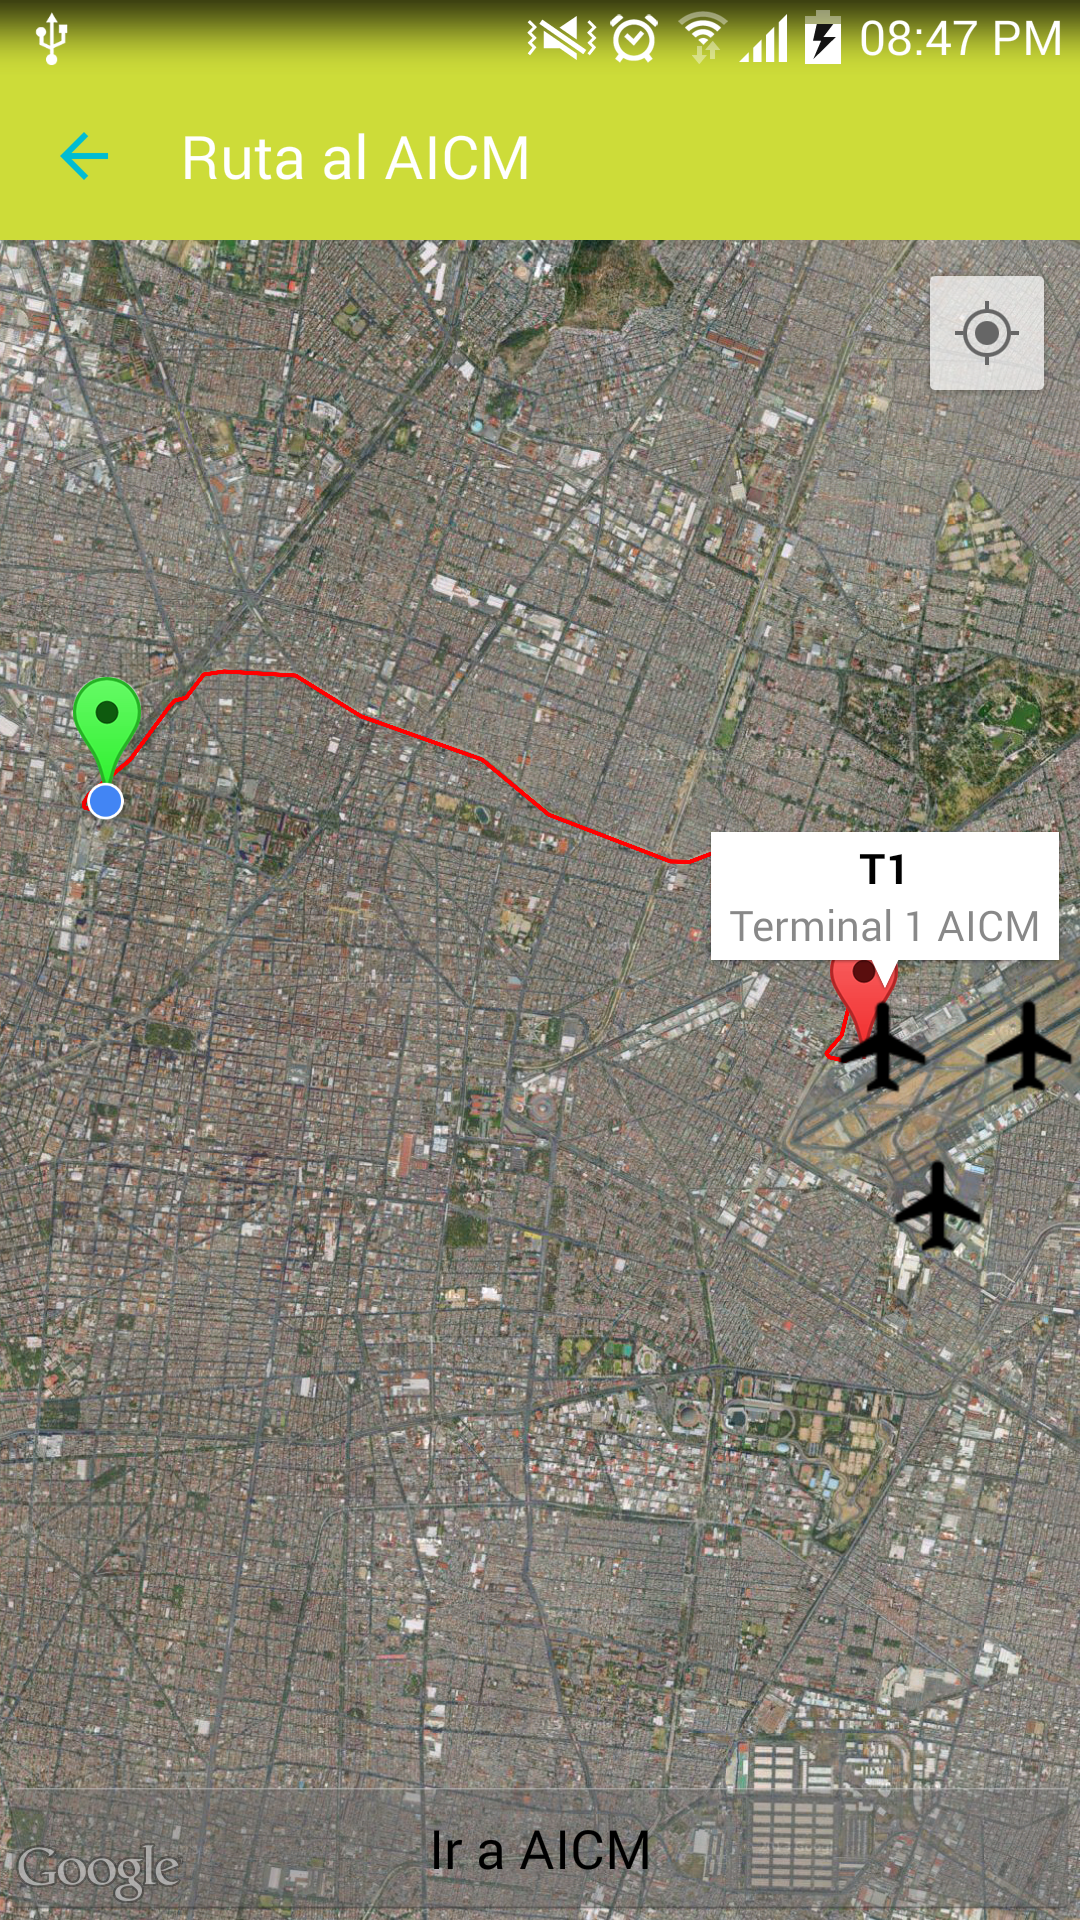
\includegraphics[width=0.5\textwidth]{Figuras/escenariot1.png}
		\rule{30em}{0.5pt}
	\caption[Escenario de prueba 1 para la generación de ruta (Terminal 1)]{Escenario de prueba 1 para la generación de ruta (Terminal 1)}
	\label{fig:vistaPruebaR1}
\end{figure}
\clearpage

\begin{figure}[h]
	\centering
		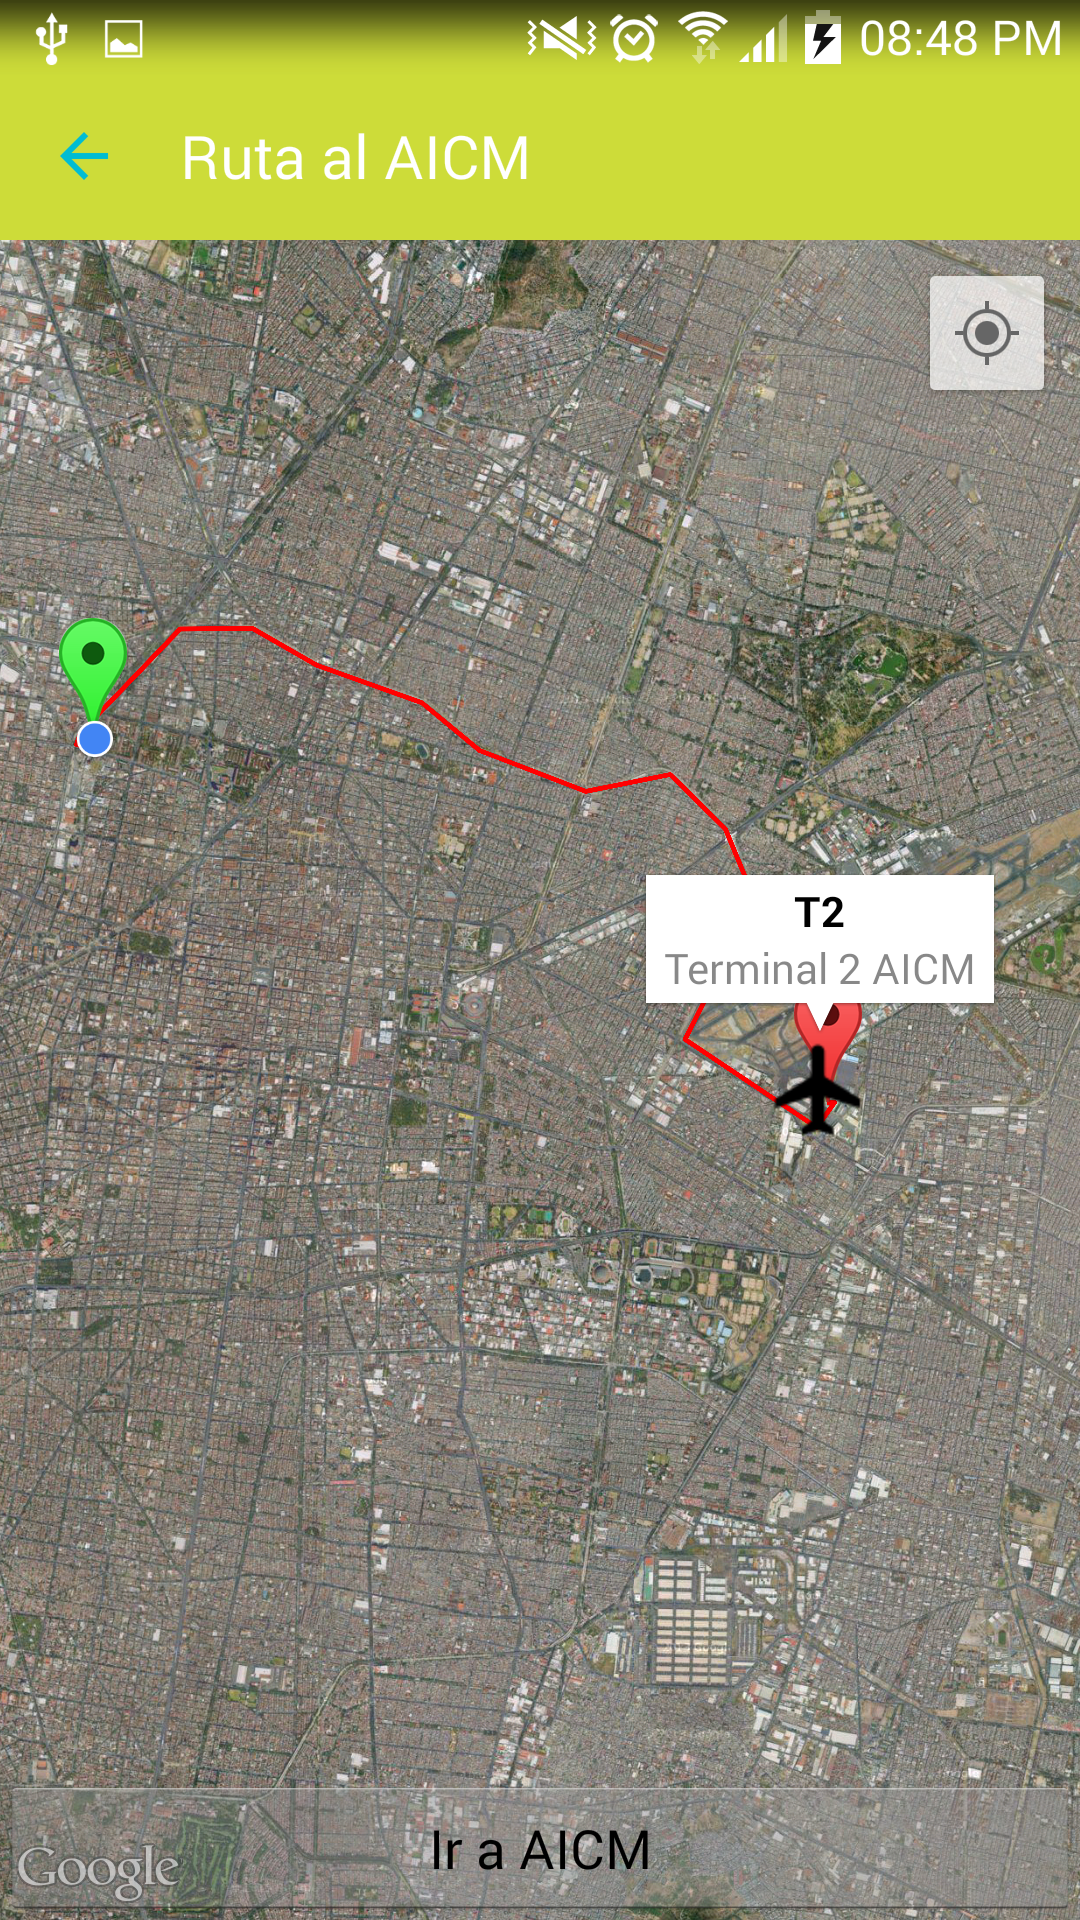
\includegraphics[width=0.5\textwidth]{Figuras/escenariot2.png}
		\rule{30em}{0.5pt}
	\caption[Escenario de prueba 2 para la generación de ruta (Terminal 2)]{Escenario de prueba 2 para la generación de ruta (Terminal 2)}
	\label{fig:vistaPruebaR2}
\end{figure}
\clearpage

\subsection{Actualización de información de hoteles disponibles}
La información de hoteles disponibles se encuentra en constante cambio por lo que es es necesario realizar una actualización de la misma, 
es por ello que mediante la implementación de un gesto táctil de deslizamiento de arriba hacia abajo, dicha información es actualizada, 
realizando una nueva petición JSON al servicio externo que brinda está información.
\begin{figure}[h]
	\centering
		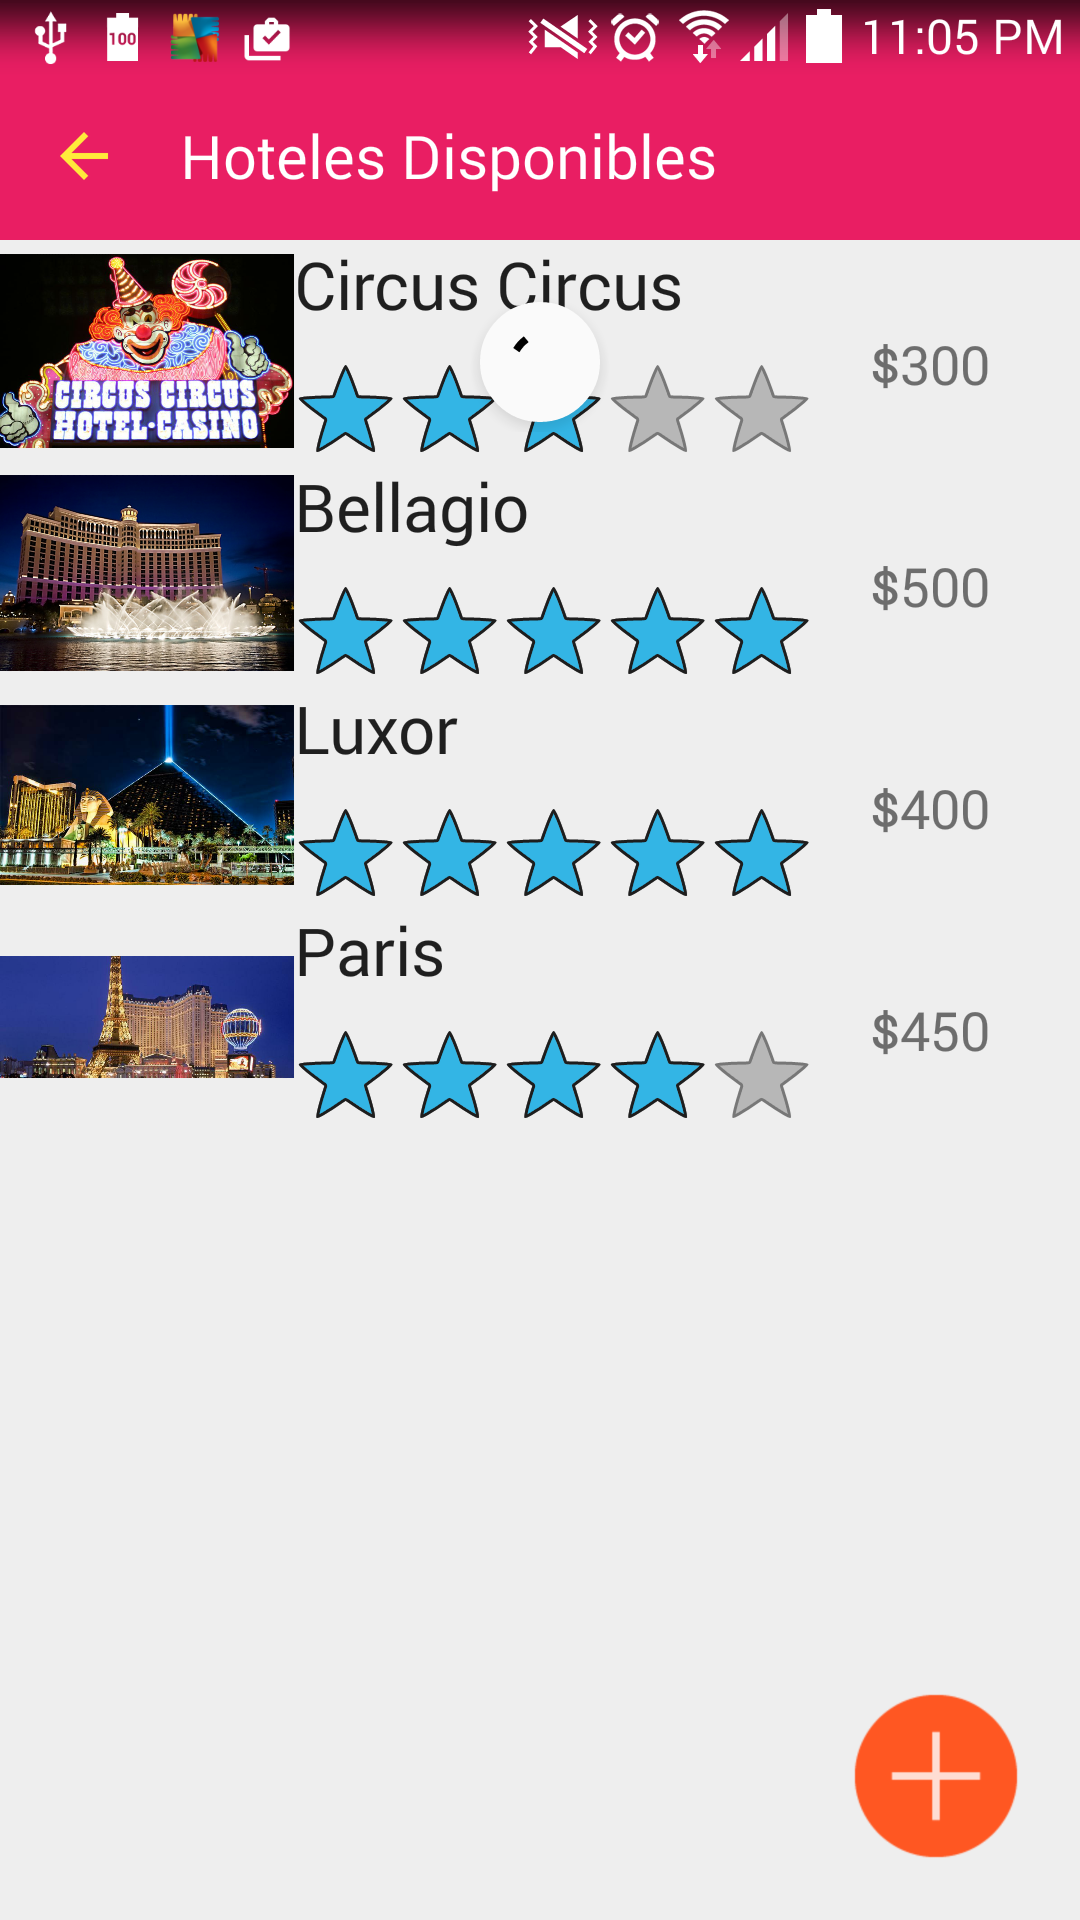
\includegraphics[width=0.5\textwidth]{Figuras/actualizaHoteles.png}
		\rule{30em}{0.5pt}
	\caption[Escenario de prueba para actualización de información de hoteles disponibles]{Escenario de prueba para actualización de informacion de hoteles disponibles}
	\label{fig:vistaPruebaActh}
\end{figure}
\clearpage

\subsection{Actualización de información de vuelos disponibles}
La información de vuelos disponibles se encuentra en constante cambio por lo que es es necesario realizar una actualización de la misma, 
es por ello que mediante la implementación de un gesto táctil de deslizamiento de arriba hacia abajo, dicha información es actualizada, 
realizando una nueva petición JSON al servicio externo que brinda está información.
\begin{figure}[h]
	\centering
		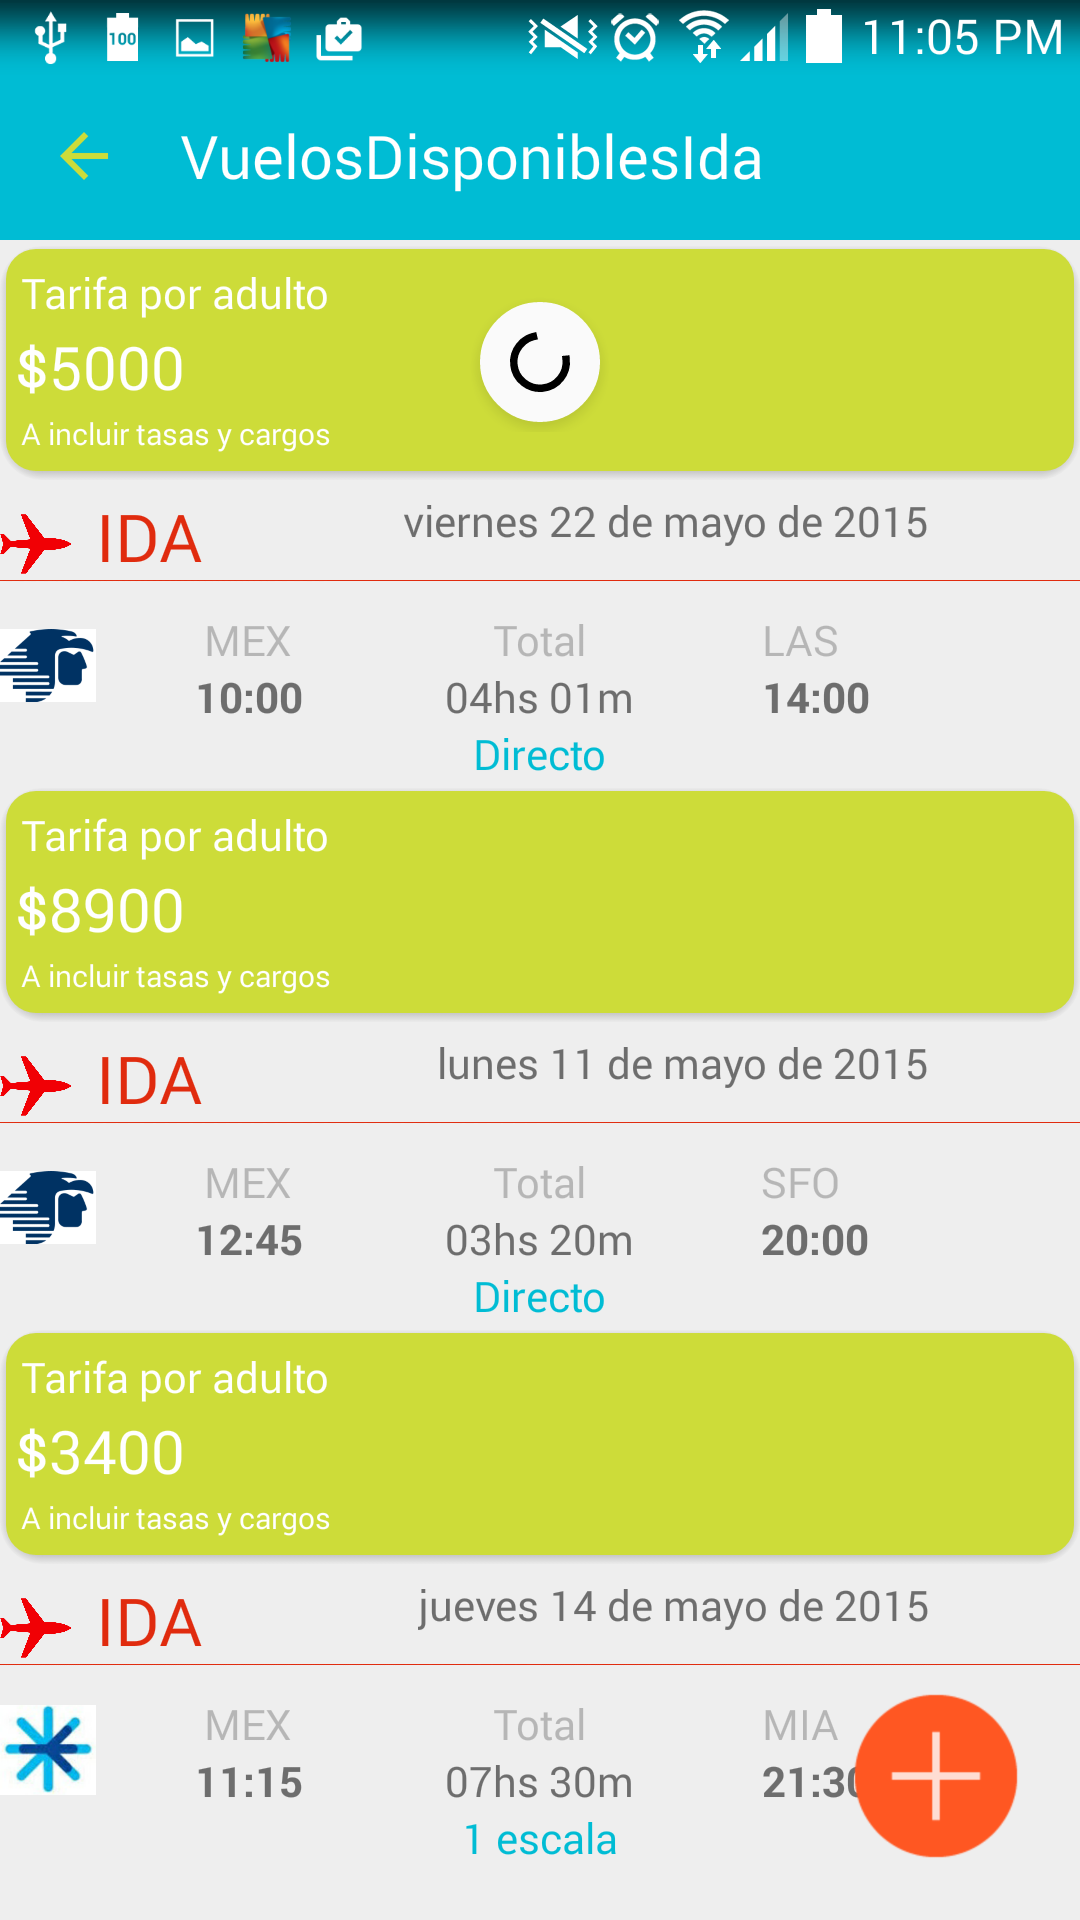
\includegraphics[width=0.5\textwidth]{Figuras/actualizaIdas.png}
		\rule{30em}{0.5pt}
	\caption[Escenario de prueba para actualización de información de vuelos disponibles (Ida)]{Escenario de prueba para actualización de informacion de vuelos disponibles (Ida)}
	\label{fig:vistaPruebaActi}
\end{figure}
\clearpage

\begin{figure}[h]
	\centering
		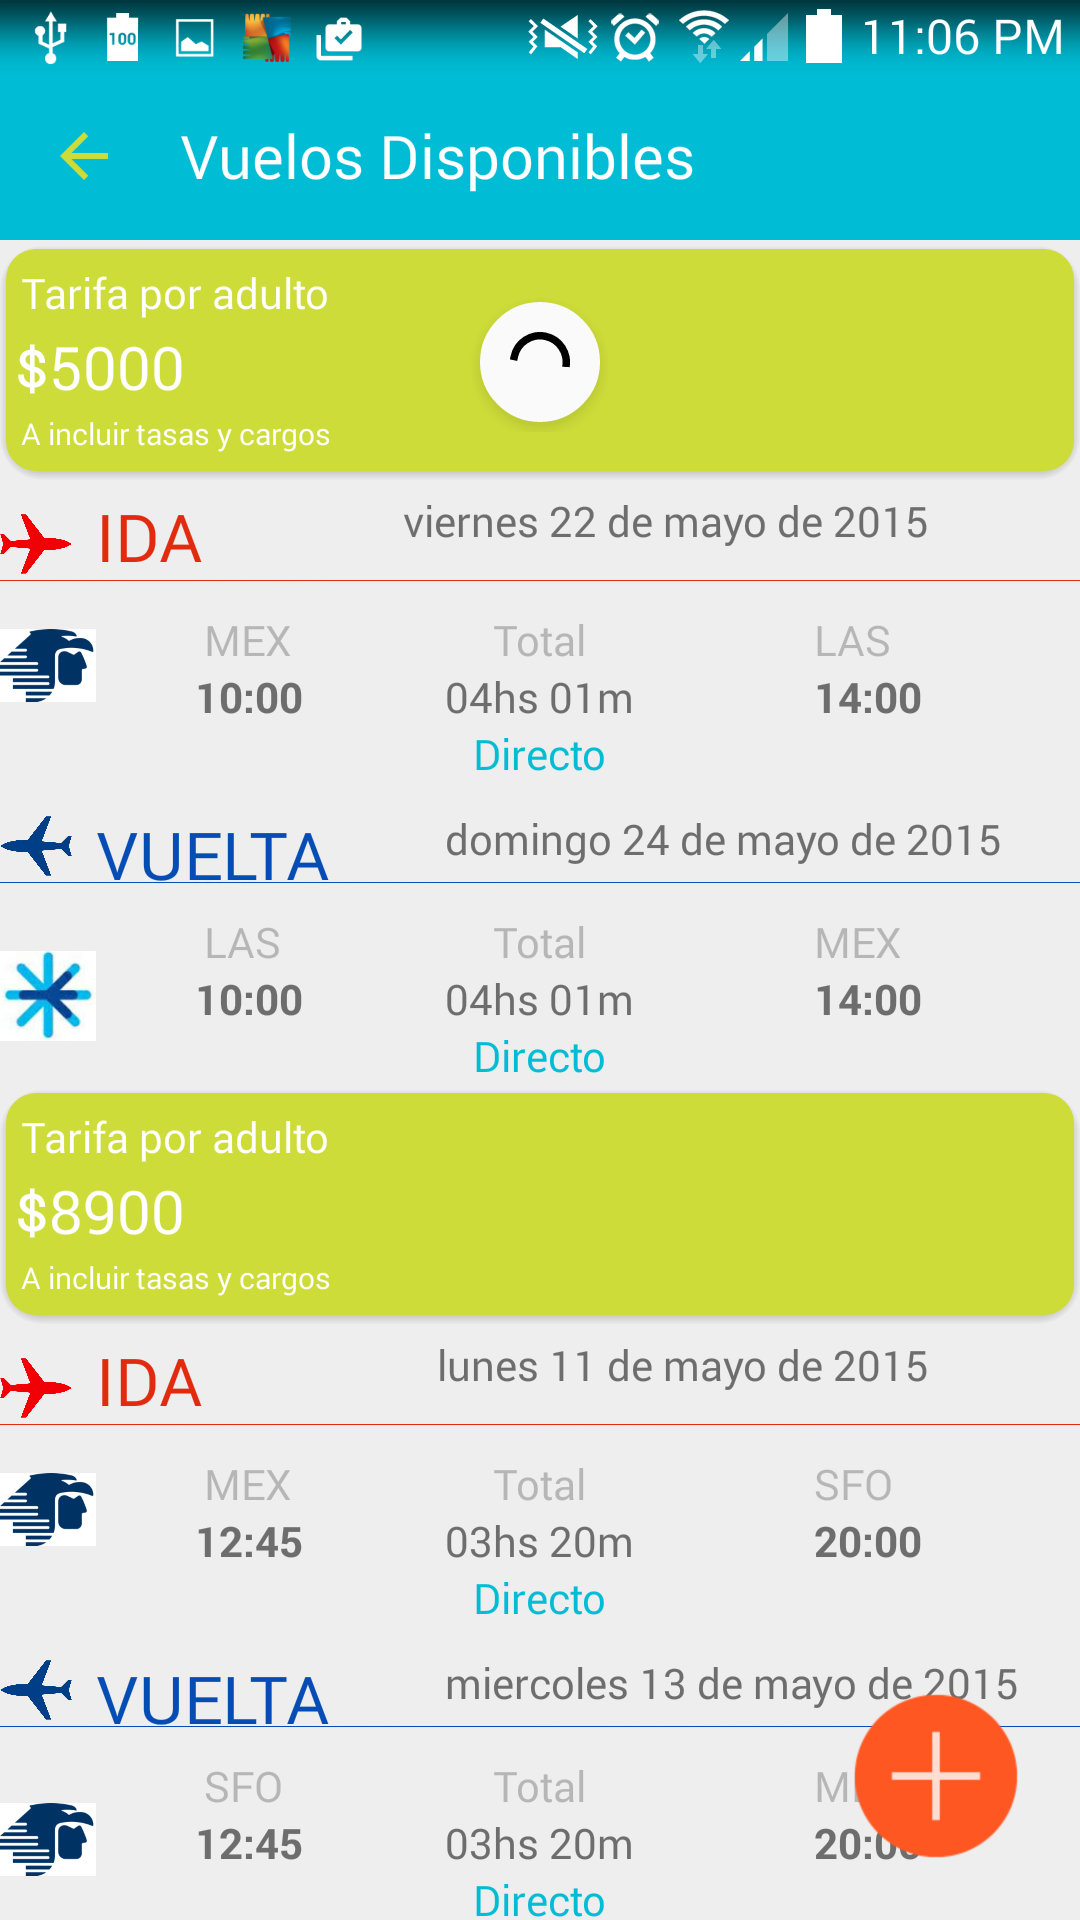
\includegraphics[width=0.5\textwidth]{Figuras/actualizaVueltas.png}
		\rule{30em}{0.5pt}
	\caption[Escenario de prueba para actualización de información de vuelos disponibles (Ida y Vuelta)]{Escenario de prueba para actualización de informacion de vuelos disponibles (Ida y Vuelta)}
	\label{fig:vistaPruebaActv}
\end{figure}
\clearpage

\subsection{Pruebas de trayectorias para la localización dentro del AICM}
Para probar el módulo de ubicate se realizaron un trazado de distintos tipos de trayectorias donde se analizó cual fue la mejor 
opción en cuestión de exactitud. 

\subsection{Trayectoria redundante}
Se trazo una trayectoria redundante con la finalidad de tener un camino que fuera de ida y vuelta. Los resultados que se obtuvieron 
fueron negativos ya que se tenía pensado que fuera redundante y se pudiera usar una trayectoria tanto de ida como vuelta.

\begin{figure}[h]
	\centering
		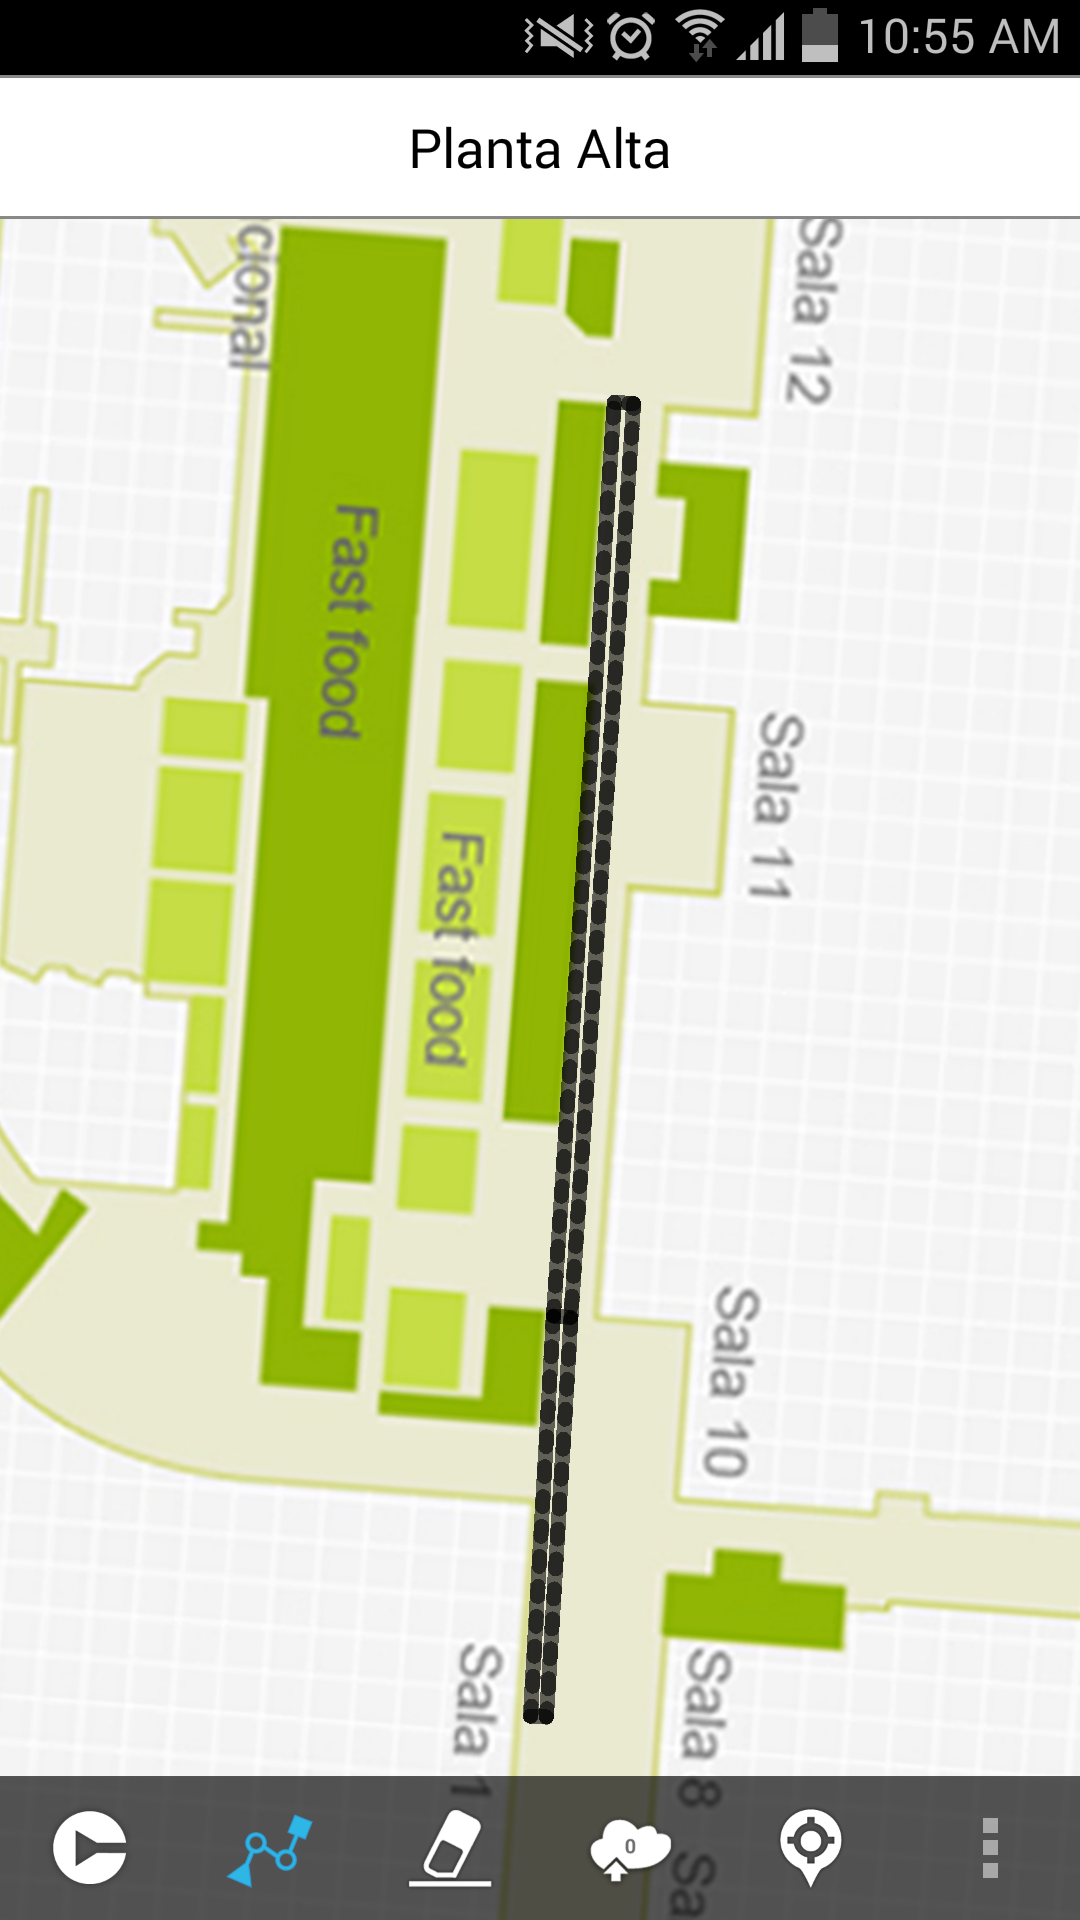
\includegraphics[width=0.5\textwidth]{Figuras/redundante.png}
		\rule{30em}{0.5pt}
	\caption[Prueba trayectoria redundante]{Prueba trayectoria redundante}
	\label{fig:vistaPruebaRedundante}
\end{figure}
\clearpage

\subsection{Trayectoria zigzag}
Se trazo una trayectoria simulando un zigzag la cual no fue efectiva pues a pesar de abarcar más área, el API utilizada guarda unicamente 
la trayectoria, no los valores magnéticos en el área.
\begin{figure}[h]
	\centering
		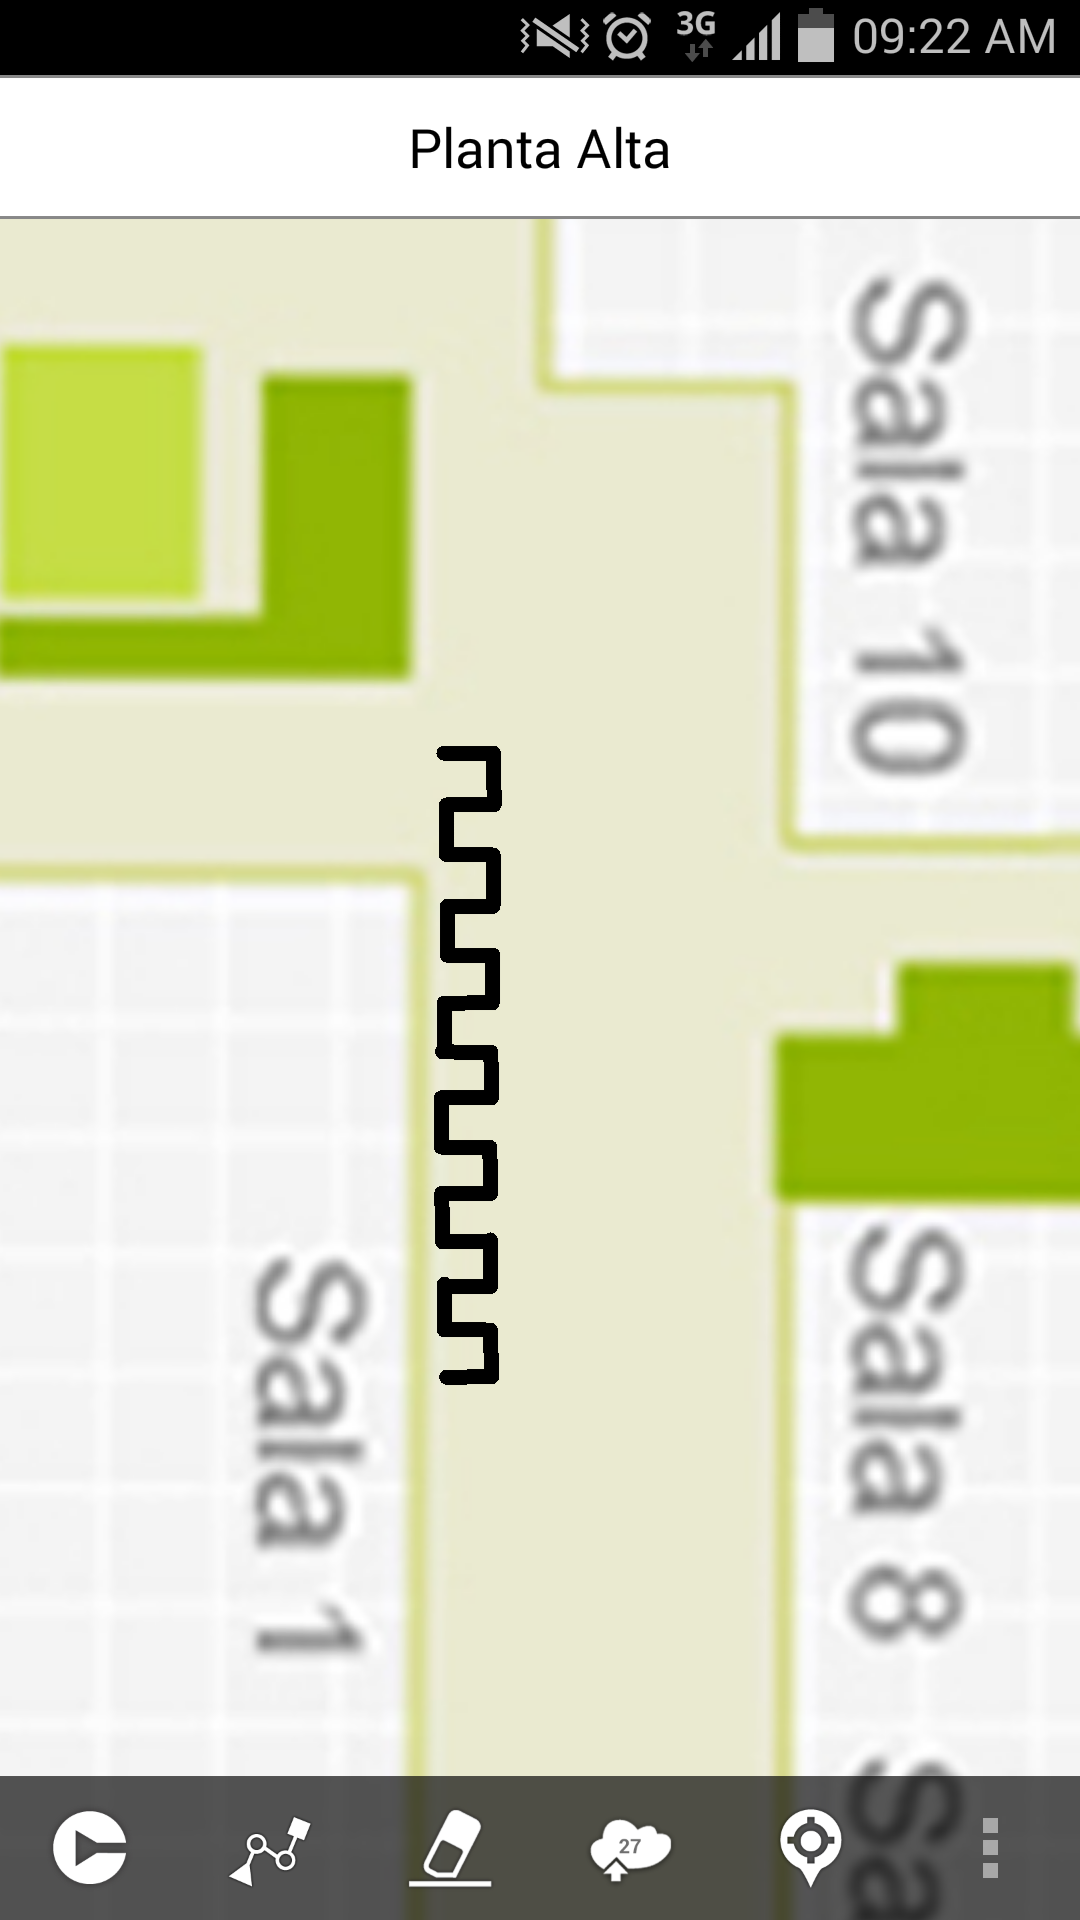
\includegraphics[width=0.5\textwidth]{Figuras/zigzag.png}
		\rule{30em}{0.5pt}
	\caption[Prueba trayectoria zigzag]{Prueba trayectoria zigzag}
	\label{fig:vistaPruebaZig}
\end{figure}
\clearpage

\subsection{Trayectoria medio backbone}
Se trazo únicamente una ruta la cual serviría de ida y vuelta, se dividio el andén de pasajeros a la mitad pensando que teniendo 
trayectorias segmentadas por cada sala de última espera se podía obtener una mayor exactitud pero los resultados de exactitud eran de cinco 
metros.
\begin{figure}[h]
	\centering
		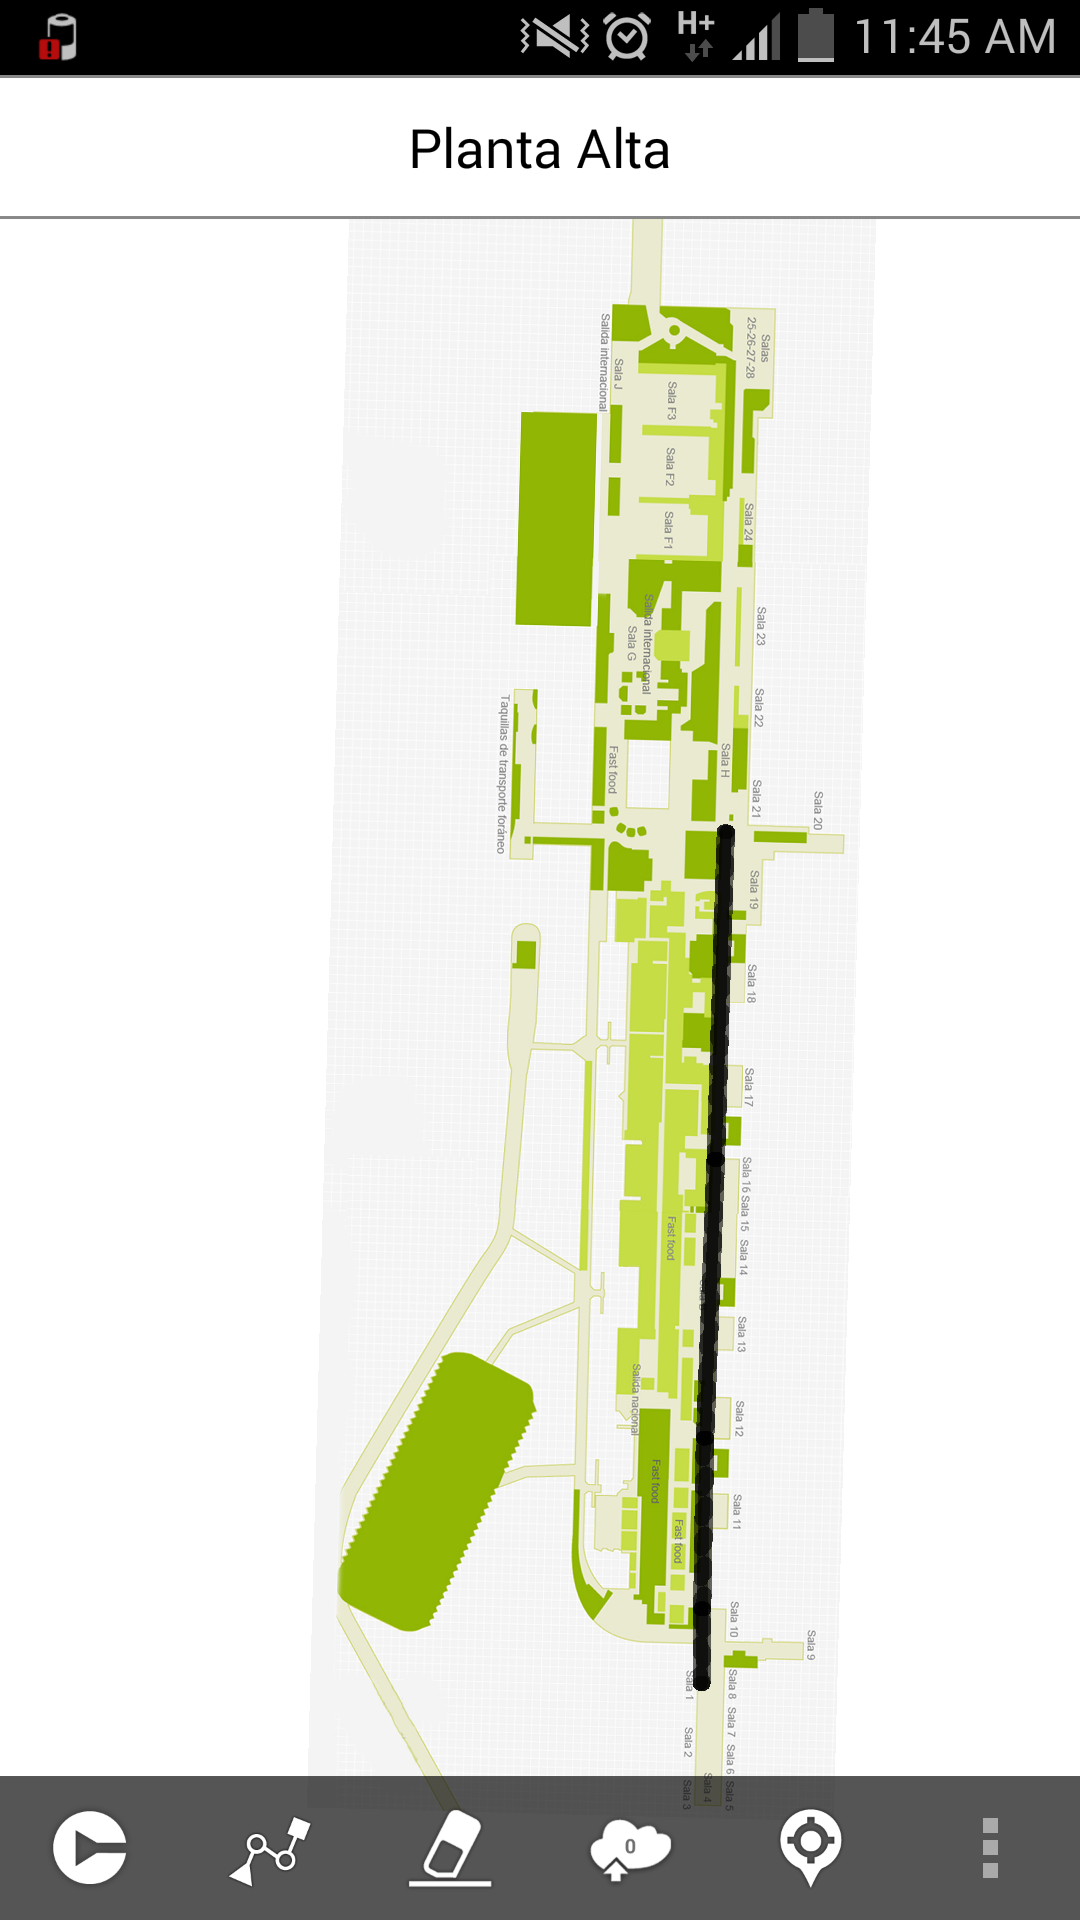
\includegraphics[width=0.5\textwidth]{Figuras/medioback.png}
		\rule{30em}{0.5pt}
	\caption[Prueba trayectoria medio backbone]{Prueba trayectoria medio backbone}
	\label{fig:vistaPruebaMedioBack}
\end{figure}
\clearpage

\subsection{Trayectoria backbone}
Finalmente se trazó un llamado backbone sobre el anden principal de pasajeros, medio por el cual se comunican las distintas salas de espera 
del AICM-T1 de está manera se obtuvieron los mejores resutados ya que se pudó obtener una exactitud de tres metros. A partir de ello 
se trazarón las distintas trayectorias en cada una de las salas de última espera.
\begin{figure}[h]
	\centering
		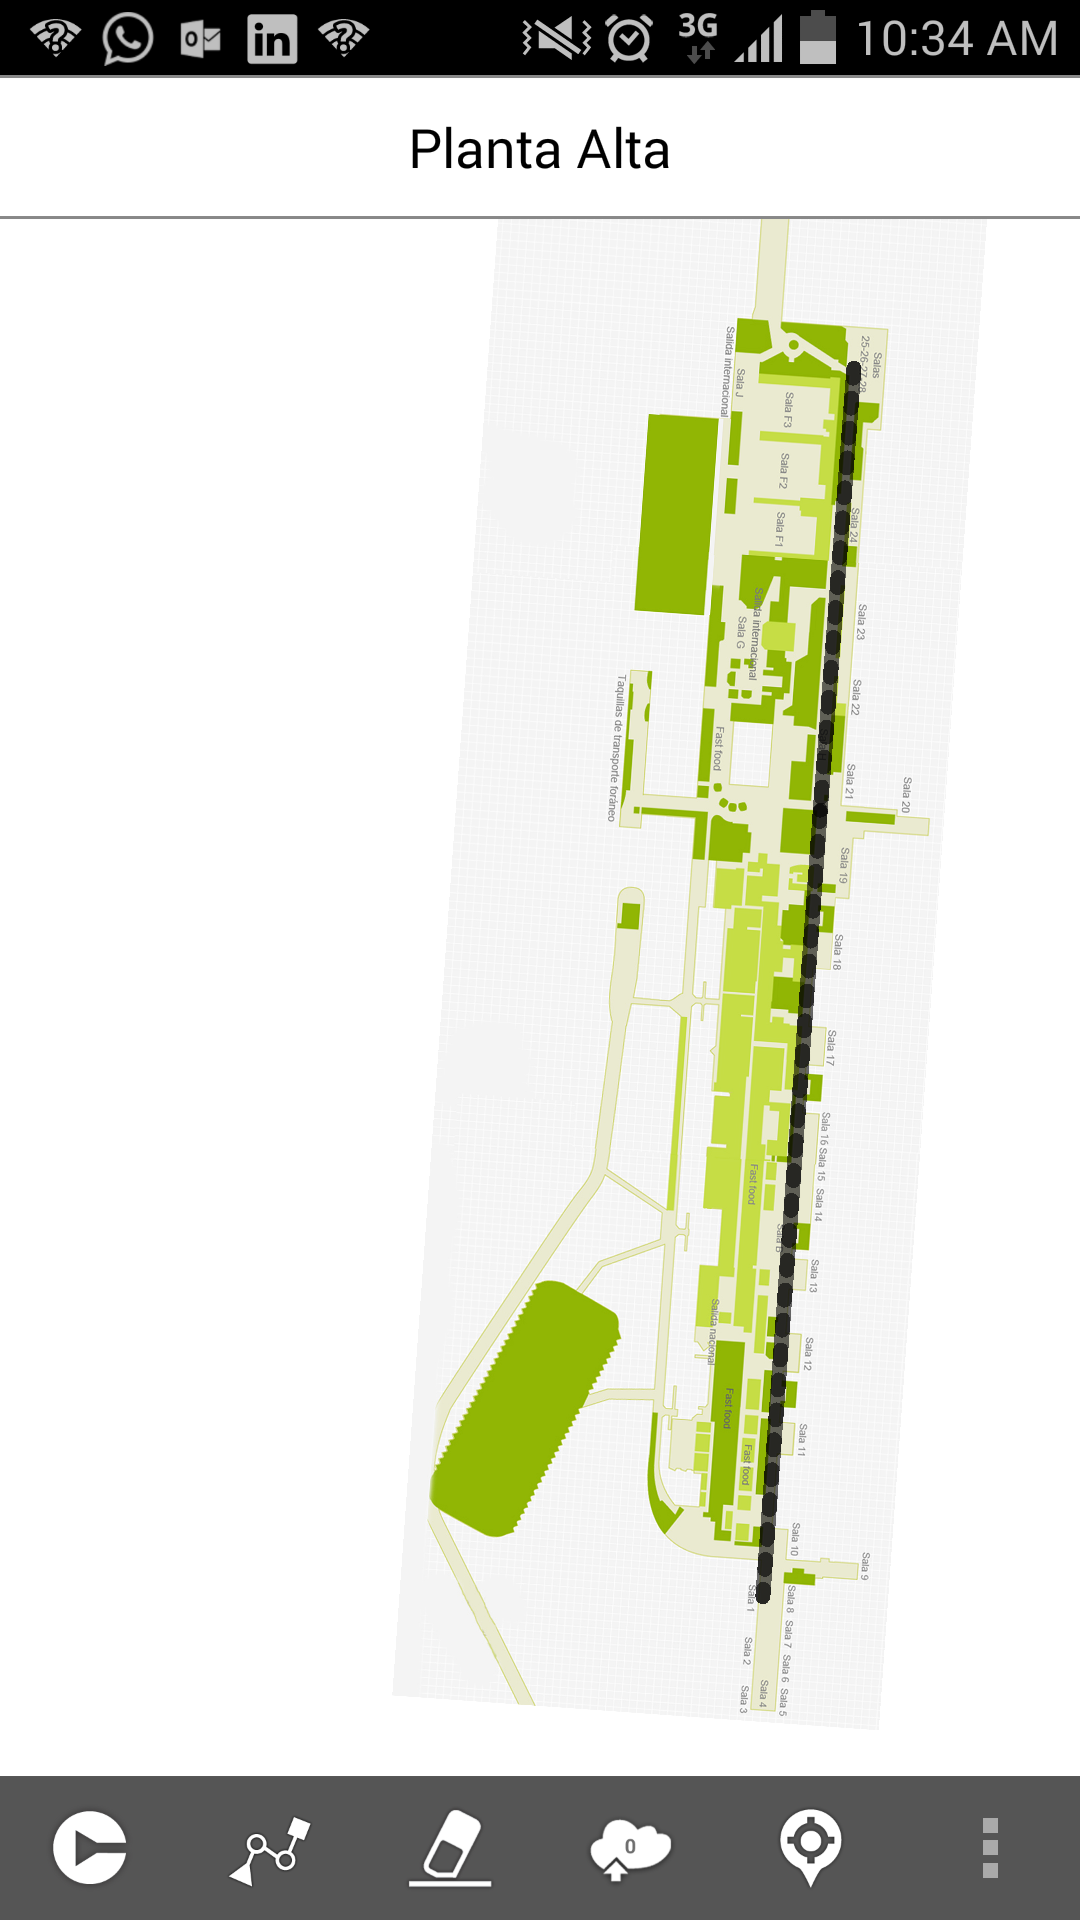
\includegraphics[width=0.5\textwidth]{Figuras/backbone.png}
		\rule{30em}{0.5pt}
	\caption[Prueba trayectoria backbone]{Prueba trayectoria backbone}
	\label{fig:vistaPruebaBackbone}
\end{figure}
\clearpage

\begin{figure}[h]
	\centering
		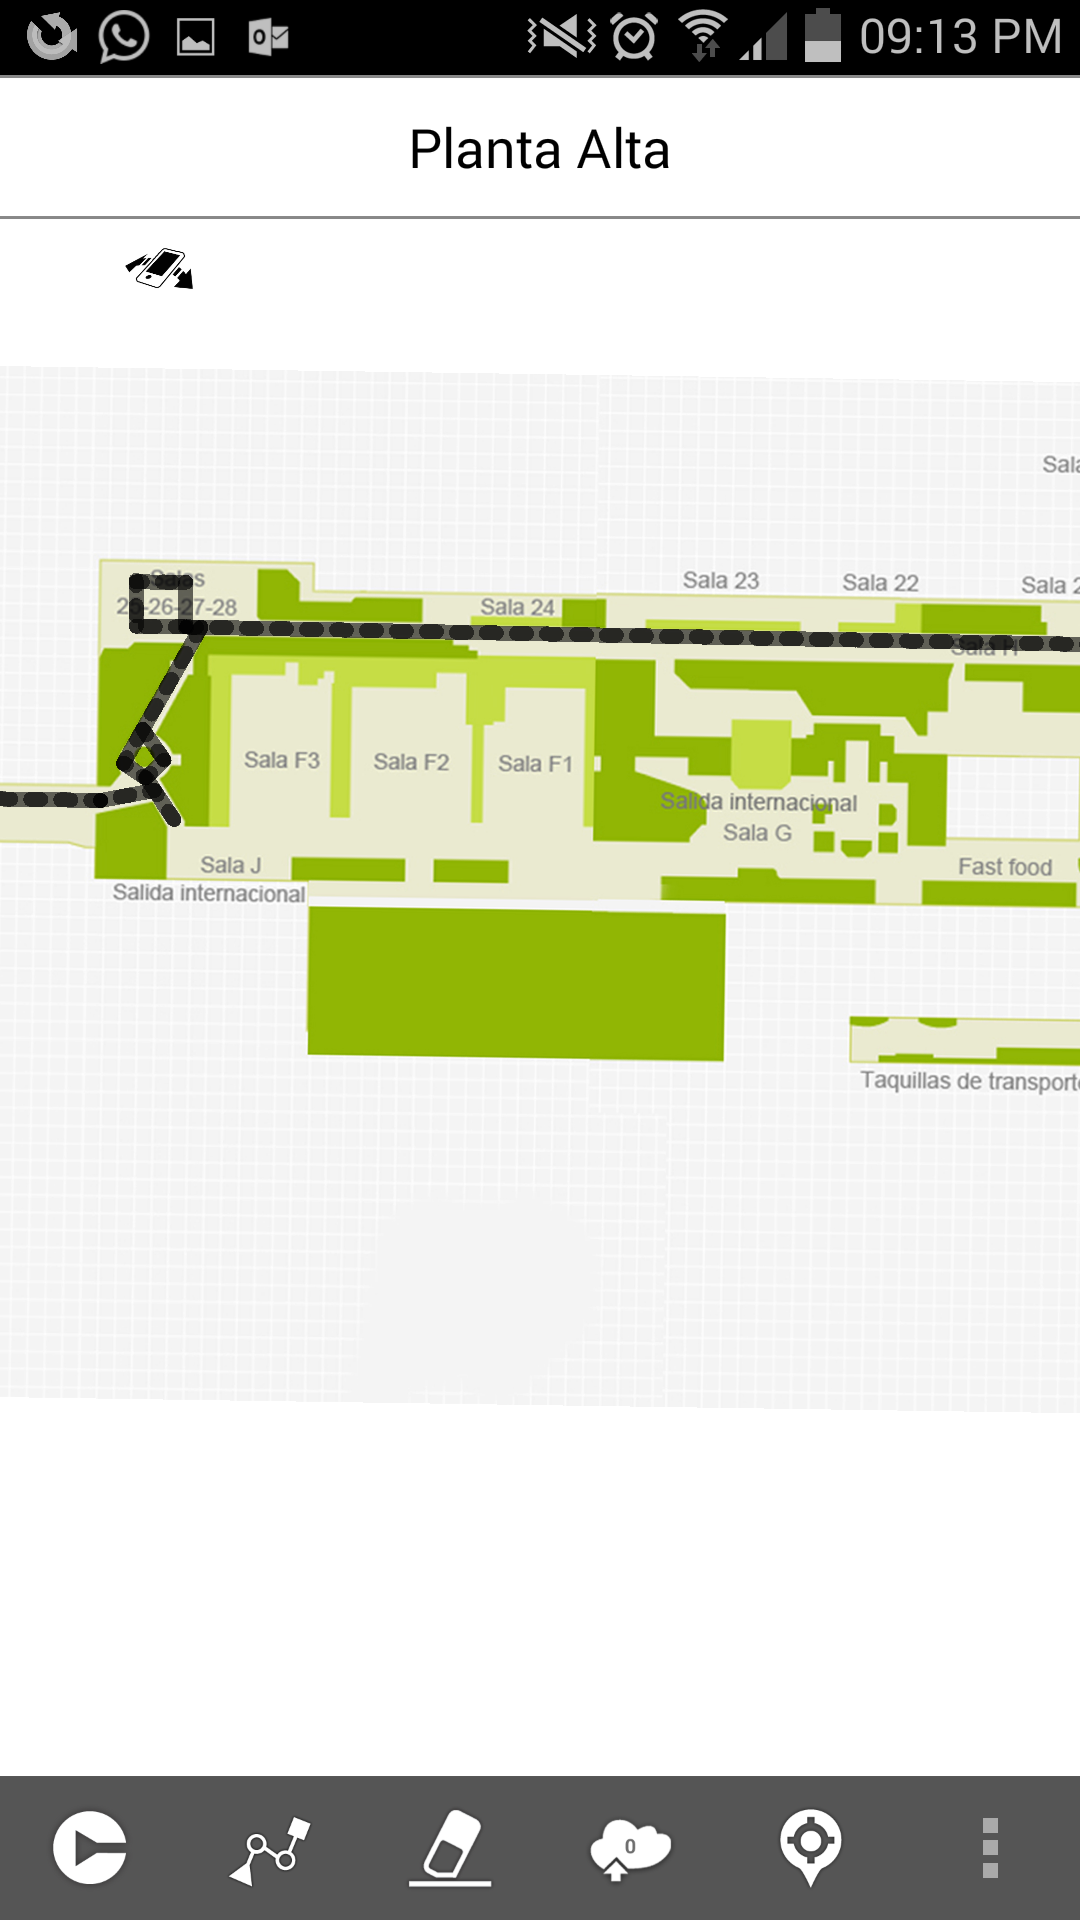
\includegraphics[width=0.5\textwidth]{Figuras/inter.png}
		\rule{30em}{0.5pt}
	\caption[Prueba trayectoria dentro de salas de última espera]{Prueba trayectoria dentro de salas de última espera}
	\label{fig:vistaPruebaSUES}
\end{figure}
\clearpage


\begin{figure}[h]
	\centering
		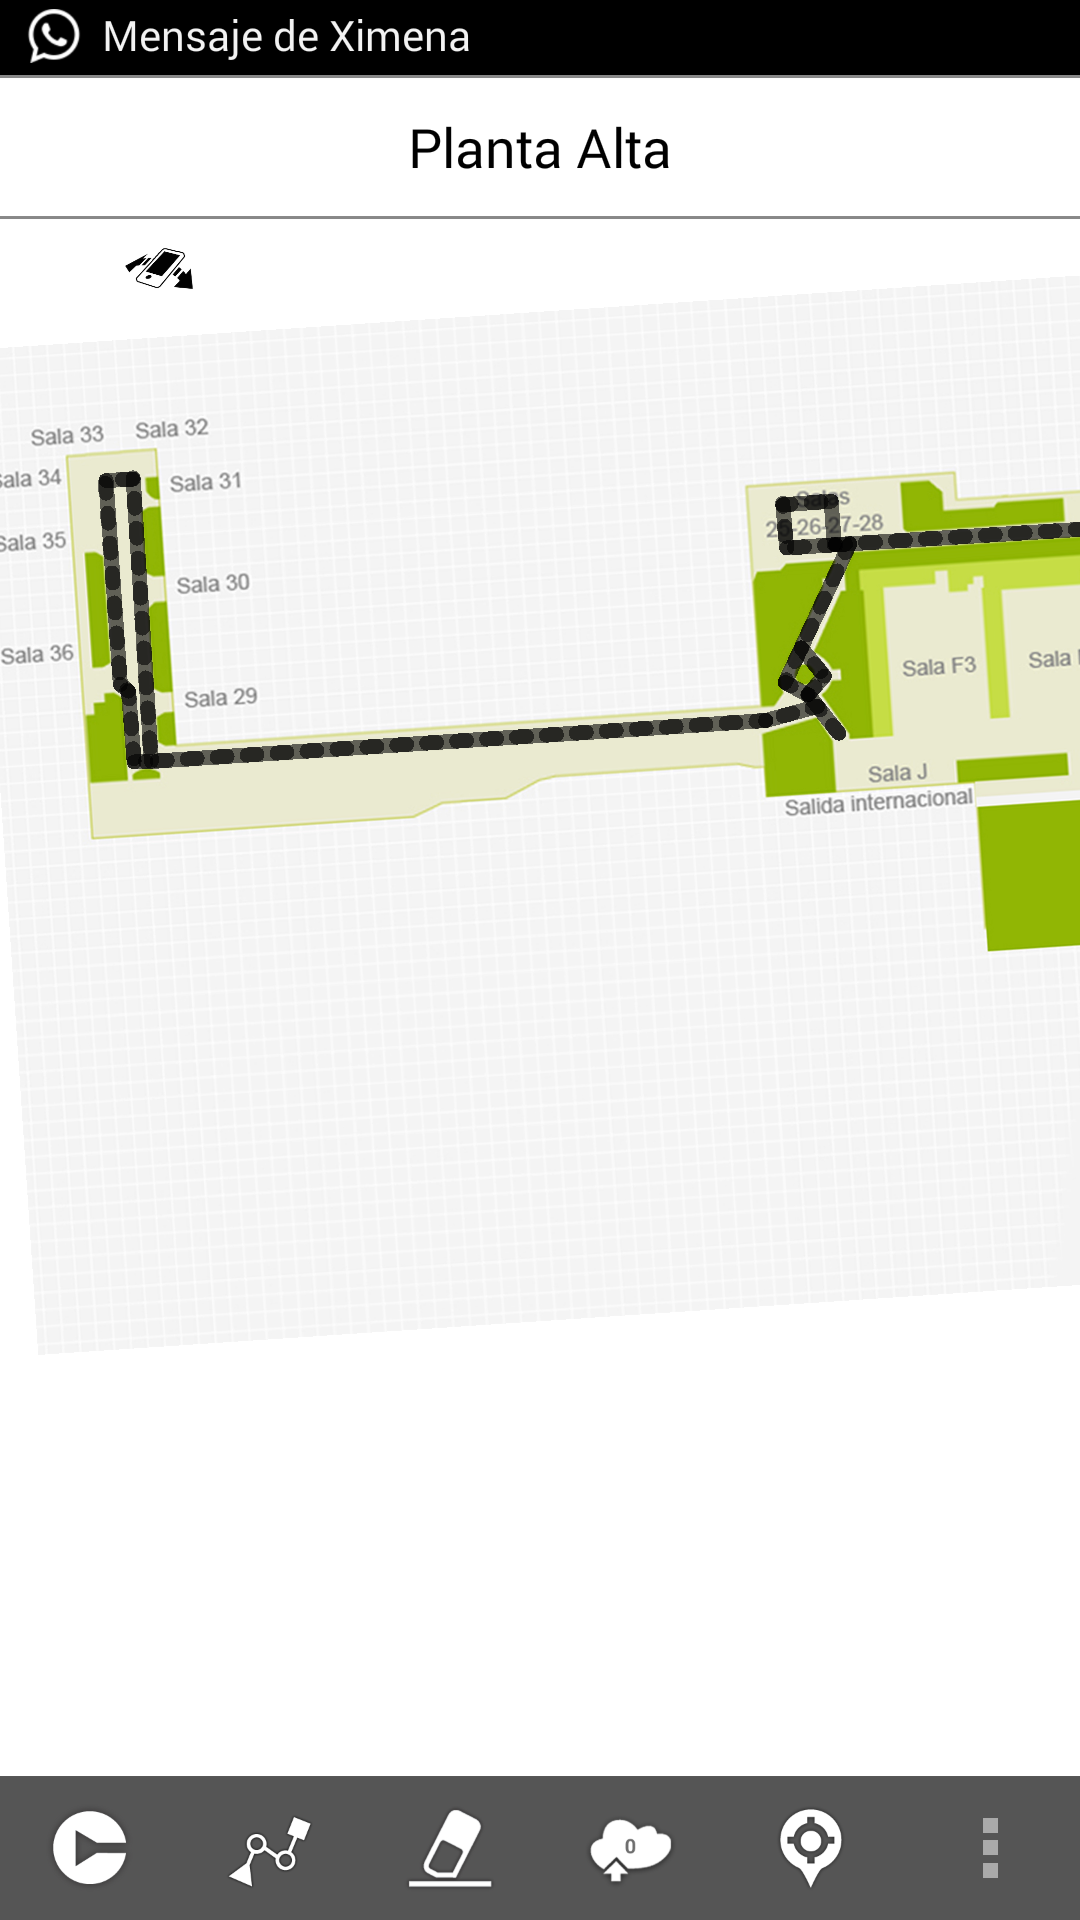
\includegraphics[width=0.5\textwidth]{Figuras/monarca.png}
		\rule{30em}{0.5pt}
	\caption[Prueba trayectoria pasillo monarca]{Prueba trayectoria pasillo monarca}
	\label{fig:vistaPruebaMonarca}
\end{figure}
\clearpage

A pesar de realizar distintas pruebas el rendimiento que obteniamos de la ubicación era de un porcentaje no tan razonable, ya que 
el API que se utiliza guarda dichas trayectorias en una nube, ente por el cuál se debe ingresar usando una conexión a Internet, 
la terminal 1 cuenta con distintas redes repartidas en las salas de espera, las cuales pierden potencia cuando uno se encuentra dentro 
del pasillo principal (anden de pasajeros), de está manera nos encontramos con distintas zonas muertas (lugares sin internet), 
mismas donde la respuesta a la ubicación en interiores iba a perder capacidad. 
Finalmente se realizaron mediciones de los valores de espectros magnéticos,los cuales son guardados en cada trayectoria trazada, 
de igual manera se encontro que dichos valores iban a ser variables dependiendo del flujo de personas, ya que ellos pueden acarrear 
distintos objetos que pueden generar variaciones al espectro magnético, de esta manera el rendimiento final que se pudó obtener utilizando 
esta API es del ochenta porciento. Es por esto que se planteá como trabajo a futuro poder montar una nueva infraestructura de sensores 
que permitan obtener una mejor respuesta.

